\documentclass[12pt,a4paper]{article}

%% Package using
\usepackage[utf8]{inputenc}
\usepackage{xeCJK}          % 使用中文
\usepackage{graphicx}       % 插入圖片
\usepackage{indentfirst}    % 首段空格
\usepackage{listings}       % code block
\usepackage{xcolor}         % set color


%% Document Style
\linespread{1.5}    % 行距    
\setCJKmainfont{NotoSansTC-Light.otf}[
Path=./Font/,
BoldFont=NotoSansTC-Regular.otf]     % 中文字型_黑體
\renewcommand{\familydefault}{\sfdefault}   % 英文字型_sans font
\renewcommand\contentsname{目錄}            % TOC標題 : Content -> 目錄
\graphicspath{{./Pic/}}                     % 圖片路徑
\setlength{\parindent}{2em}                 % 首段空兩格


% Code block style
\definecolor{gray}{rgb}{0.5,0.5,0.5}
\definecolor{backColor}{HTML}{f7f6f2}
\definecolor{darkgreen}{HTML}{7f9353}
\definecolor{darkblue}{HTML}{629aaa}
\definecolor{darkred}{HTML}{d38696}

\lstset{
  inputpath=../,
  language=Matlab,
  basicstyle={\linespread{1.0}\ttfamily\small},
  backgroundcolor=\color{backColor},
  keywordstyle=\color{darkblue},
  identifierstyle=\color{darkred},
  commentstyle=\color{gray},
  stringstyle=\color{darkgreen},
  showstringspaces=false,
  keepspaces=true,
  columns=flexible,
  breaklines=true,
  breakatwhitespace=true,
  tabsize=4,
%   numbers=left,
%   stepnumber=1
}


%% Document Content
\begin{document}

% Title page
\begin{center}
    
    \vspace*{5cm}
    \textbf{\huge Orientation Homework Report}\\   % 粗體+加大
    
    \vspace{1cm}
    {\large 10-bar truss optimization}
    
    \vfill
    {\Large 徐若瑄}
    
    \vspace{1cm}
    {\Large \today}

\end{center}
\newpage

% %----------------Next Page--------------

% \tableofcontents

% \newpage
% %----------------Next Page--------------

% Section 1
\section{問題描述}

    十桿衍架(10-bar truss)由十個長桿件組成並且有6個端點,其中第5、6號端點為固定端,桿件的配置如圖\ref{10-bar truss}所示。
    
    \begin{figure}[h]
        \centering
        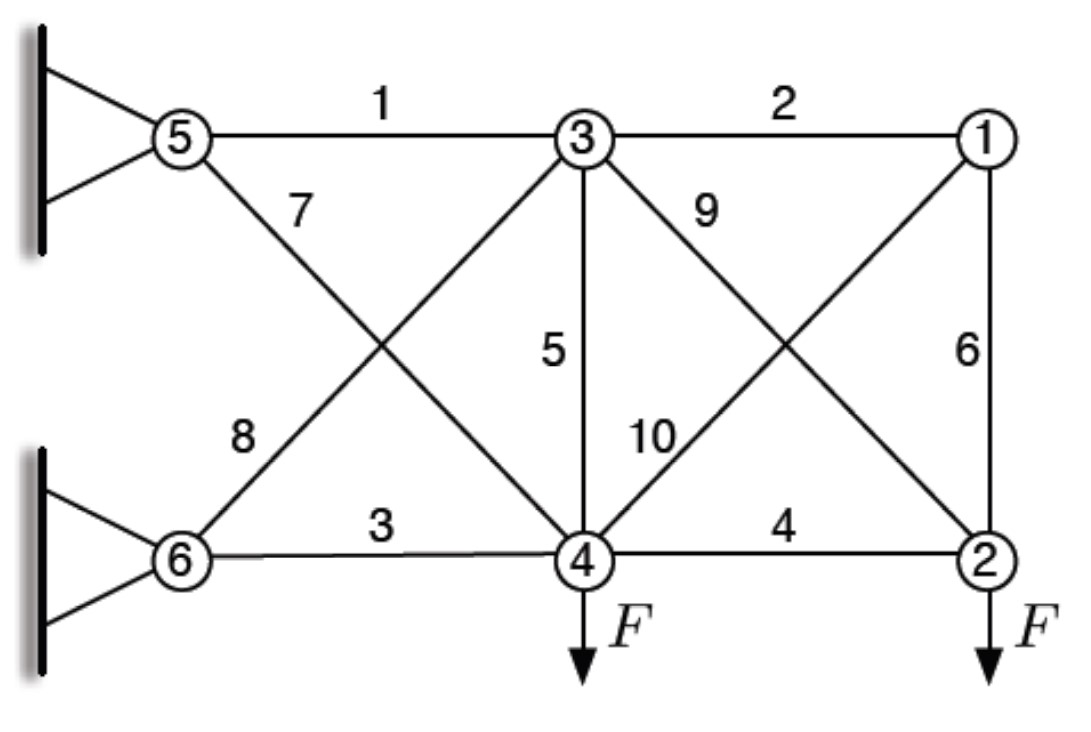
\includegraphics[width=8cm]{10_bar_truss}
        \caption{10-bar truss}
        \label{10-bar truss}
    \end{figure}
    
    所有桿件的截面皆為圓形,桿件1到桿件6的截面半徑同為$r1$且長度為$9.14\  m$;桿件7到桿件8的截面半徑同為$r2$。
    桿件所使用的材料為剛,相關的材料性質有:
    
    \begin{enumerate}
        \item 密度 $\rho = 7860\ kg/m^3$
        \item 楊氏模數(Young's Modulus) $E = 200\ GPa$
        \item 降伏係數(Yield stress) $\sigma_y = 250\ MPa$
    \end{enumerate}
    
    端點4及端點5有一向下的外力$F = 1.0x10^-7\ N$,
    在所有桿件的應力不超過降伏應力且端點2的位移小於$0.02\ m$的條件下,
    求桿件截面半徑$r1$與$r2$的值,使得十桿衍架整體重量為最輕。
    
\newpage
%----------------Next Page--------------

% Section 2
\section{計算方法}
    
    計算十桿衍架最小重量主要使用兩個方法,首先利用有限元素法(Finite element method)計算出所有桿件的應力值、各個端點的位移量,接著進行最佳化即可得到最佳值與最佳解。
    
    以下所有計算過程皆使用Matlab程式輔助計算。
    
    \subsection{有限元素分析}
        
        有限元素分析的關鍵步驟如下:
        \begin{enumerate}
            \item 建立元素表(Element Table):
                  元素表內包含各桿件的長度、截面積、角度等
            \item 建立剛性矩陣(Stiffness Matrix):
                  利用元素表計算出剛性矩陣$K$,表示出6個端點的12個自由度上下位移與受力之間的關係
            \item 計算各個節點的位移:
                  透過$F=KQ$的關係式求出各點在x,y兩方向的位移量
            \item 計算各桿件的應力:
                  透過$\sigma=E\varepsilon$的關係式求出各桿件的應力
            \item 計算反作用力:
                  同樣使用$F=KQ$的關係式求出固定端點5、6的反作用力
            \item 最佳化:
                  將問題條件轉換為數學式,最佳化後得到最佳值與最佳解
        \end{enumerate}
        
        \newpage
%----------------Next Page--------------

        \subsubsection{建立端點與桿件參數}
        
            為了快速建立元素表,首先將桿件長度轉換為各端點的座標位置(以端點6為原點)並存於\texttt{nodeTable}
            \lstinputlisting[firstline=10,lastline=16]{finiteElementMethod.m}
            
            接著設定桿件1到桿件10對應到的左右兩截點編號。
            利用\texttt{nodeInfo}紀錄各端點連接的桿件編號,
            再將桿件兩端點的編號存於\texttt{elementToNode}
            \lstinputlisting[firstline=18,lastline=29]{finiteElementMethod.m}
            

        \subsubsection{建立元素表}
            
            元素表\texttt{elementTable} 為10x4的矩陣,
            每一欄依序紀錄各桿件的長度$L$、截面積$A$、$cos$及$sin$。
            以\texttt{elementToNode}搭配\texttt{nodeTable}計算各項數值
            \lstinputlisting[firstline=41,lastline=67]{finiteElementMethod.m}

\newpage
%----------------Next Page--------------

% Section 3
\section{結論}

\end{document}
